\section{Introduction}


%Distributed and collaborative machine learning has been widely studied in order to handle exploding amount of data.

The effectiveness of a machine learning model does not only depend on the quantity of samples, but also the quality of data, especially the availability of high-quality features.
Recently, a wide range of distributed and collaborative machine learning schemes, including gradient-based methods \cite{li2014communication,ho2013more} and ADMM-based methods \cite{zhang2018improving,zhang2016dual,huang2018dp},
have been proposed to enable learning from distributed samples, since collecting data for centralized learning will incur compliance overhead, privacy concerns, or even judicial issues. Most existing schemes, however, are under the umbrella of \emph{data parallel} schemes, where multiple parties possess different training samples, each sample with the same set of features. 
%are under the umbrella of \emph{data parallel} schemes.
For example, different users hold different images to jointly train a classifier.

An equally important scenario is to collaboratively learn from distributed features, where multiple parties may possess different features about a same sample, yet do not wish to share these features with each other. Examples include a user's behavioural data logged by multiple apps, a patient's record stored at different hospitals and clinics, a user's investment behavior logged by multiple financial institutions and government agencies and so forth. The question is---how can we train a joint model to make predictions about a sample leveraging the potentially rich and vast features possessed by other parties, without requiring different parties to share their data to each other?

The motivation of gleaning insights from vertically partitioned data dates back to association rule mining \cite{vaidya2002privacy,vaidya2003privacy}. A few very recent studies \cite{lou2018uplink,kenthapadi2013privacy,ying2018supervised,hu2019fdml,heinze2017preserving,dai2018privacy,bellet2015distributed} have reinvestigated vertically partitioned features under the setting of distributed machine learning, which is motivated by the ever-increasing data dimensionality as well as the opportunity and challenge of cooperation between multiple parties that may hold different aspects of information about the same samples. %These studies also differ from model parallelism \cite{zhou2016convergence}

In this paper, we propose an ADMM algorithm to solve the empirical risk minimization (ERM) problem, a general optimization formulation of many machine learning models visited by a number of recent studies on distributed machine learning  \cite{ying2018supervised,chaudhuri2011differentially}. We propose an ADMM-sharing-based distributed algorithm to solve ERM, in which each participant does not need to share any raw features or local model parameters to other parties. Instead, each party only transmits a single value for each sample to other parties, thus largely preventing the local features from being disclosed. 
% workshop change
% \emph{We establish theoretical convergence guarantees and iteration complexity results under the non-convex loss in a fully parallel setting, whereas previously, the convergence of ADMM sharing algorithm for non-convex losses is only known for the case of sequential (Gauss-Seidel) execution \cite{hong2016convergence}.

To further provide privacy guarantees, we present a privacy-preserving version of the ADMM sharing algorithm, in which the transmitted value from each party is perturbed by a carefully designed Gaussian noise to achieve
the notion of $\epsilon,\delta$-differential privacy \cite{dwork2008differential,dwork2014algorithmic}. For distributed features, the perturbed algorithm ensures that the probability distribution of the values shared is relatively insensitive to any change to a single feature in a party's local dataset.
  %We theoretically show that the privacy cost of executing $T$ epochs of the algorithm is ... \red{say something interesting here}.
Experimental results on two realistic datasets suggest thatour proposed ADMM sharing algorithm can converge efficiently. Compared to the gradient based method, our method can scale as the number of features increases and yields robust convergence. The algorithm can also converge with moderate amounts of Gaussian perturbation added, therefore enabling the utilization of features from other parties to improve the local machine learning task.
%It has also been reported that the volume and quality of data determines the upper bound of machine learning model performance.
%As a result, a number of distributed machine learning techniques have been proposed to collaboratively train a model by letting each party perform local model updates and exchange locally computed gradients  \cite{shokri2015privacy} or model parameters \cite{mcmahan2016communication} with the central server to iteratively improve model accuracy. Most of the existing schemes, however, fall into the range of \emph{data parallel} computation, where the training samples are located on different parties. For example, different users hold different images to jointly train a classifier. Different organizations may contribute their individual corpora to learn a joint language model.
\subsection{Related Work}
{\bf Machine Learning Algorithms and Privacy.} \cite{chaudhuri2009privacy}
is one of the first studies combing machine learning and differential privacy (DP), focusing on logistic regression. \cite{shokri2015privacy} applies a variant of SGD to collaborative deep learning in a data-parallel fashion and introduces its variant with DP. \cite{abadi2016deep} provides a stronger differential privacy guarantee for training deep neural networks using a momentum accountant method. \cite{pathak2010multiparty,rajkumar2012differentially} apply DP to collaborative machine learning, with an inherent tradeoff between the privacy cost and utility achieved by the trained model. Recently, DP has been applied to ADMM algorithms to solve multi-party machine learning problems \cite{zhang2018improving,zhang2016dual,zhang2019admm,zhang2017dynamic}. 

However, all the work above is targeting the data-parallel scenario, where samples are distributed among nodes. The uniqueness of our work is to enable privacy-preserving machine learning among nodes with vertically partitioned features, or in other words, the feature-parallel setting, which is equally important and is yet to be explored. 

%Aside from the distributed optimization approach mentioned above, 
Another approach to privacy-preserving machine learning is through
encryption \cite{gilad2016cryptonets,takabi2016privacy,kikuchi2018privacy} or secret sharing \cite{mohassel2017secureml,wan2007privacy,bonte2018privacy}, so that models are trained on encrypted data. However, encryption cannot be generalized to all algorithms or operations, and incurs additional computational cost.

{\bf Learning over Distributed Features.}
\cite{gratton2018distributed} applies ADMM to solve ridge regression.
\cite{ying2018supervised} proposes a stochastic learning method via variance reduction. \cite{zhou2016convergence} proposes a proximal gradient method and mainly focuses on speeding up training in a model-parallel scenario. These studies do not consider the privacy issue. \cite{hu2019fdml} proposes a composite model structure that can jointly learn from distributed features via a SGD-based algorithm and its DP-enabled version, yet without offering theoretical privacy guarantees. Our work establishes $(\epsilon,\delta)$-differential privacy guarantee result for learning over distributed features. Experimental results further suggest that our ADMM sharing method converges in fewer epochs than gradient methods in the case of high dimensional features. This is critical to preserving privacy in machine learning since the privacy loss increases as the number of epochs increases \cite{dwork2014algorithmic}. Another closely related work is based on the Frank-Wolfe algorithm~\cite{bellet2015distributed,lou2018uplink}, which is shown to be efficient for sparse features. In contrast, our ADMM sharing approach is more efficient for dense features and scales much better as the number of features grows, as will be explained in Sec.~\ref{sec:admmSharing}. %is proportional to $O\sqrt{T}$, T being the number of epochs.

% workshop change
{\bf Querying Vertically Partitioned Data Privately.} \cite{vaidya2002privacy,dwork2004privacy} are among the early studies that investigate the privacy issue of querying vertically partitioned data. \cite{kenthapadi2013privacy} adopts a random-kernel-based method to mine vertically partitioned data privately. These studies provide privacy guarantees for simpler static queries, while we focus on machine learning jobs, where the risk comes from the shared values in the optimization algorithm. Our design simultaneously achieves minimum message passing, fast convergence, and a theoretically bounded privacy cost under the DP framework.

% extract the task related information via training a machine learning model.

% \cite{heinze2017preserving} adopts a random projection method for the data set where number of features is greater than the number of samples. They first project the local features on to some rand linear space of lower dimension and calibrate it with noise. These data are shared directly to train linear machine learning models. all the above. We propose an interactive machine learning algorithm to extract the task related information from the vertically distributed data.


% We propose an efficient solution for the real application where features are distributed. In distributed machine learning system, convergence is a comprehension results of computation and communication. \red{In the case, ADMM sharing is a best fit since it is fast to converge in terms of epochs, which requires less privacy budget given certain accuracy.}

% {\bf Important references}\\
% \cite{huang2018dp} sublinear convergence rate. Due to linear approximation with a increasing strength for the quadratic term, convergence is guaranteed. Sensitivity is also decreasing. In the end, a decreased matching strength of noise is added.

% \cite{bellet2017personalized} Optimized noise budget. Not admm.

% \cite{shi2014linear}




 % Privacy-preserving technique in distributed machine learning is one of the keys to encourage data sharing in distributed system. There are mainly two lines of works in privacy-preserving, encryption and differential privacy. Although encryption based methods \cite{} have strong guarantee for data security, it has heavy computation overhead, which is not scalable. %Differential privacy (DP) based methods are light weighted. Well designed DP algorithm can achieve good model performance under certain privacy guarantee.

% Most existing DP distributed machine learning works focus on data parallel scenario, where different subsets of the samples are distributed.
% {\bf Differential Privacy Machine Learnings}\\
% \cite{zhang2018improving} latest result for DP ADMM work. In this work, a modified version of ADMM where the penalty and the dual variable step size is decoupled as long as the penalty is increasing over the iterations and the penalty is greater than the dual variable step size. It is shown to converge in this modified ADMM. Further more, perturbation is applied on the penalty to guarantee the privacy.



% \begin{figure}[t]
%     \centering
%     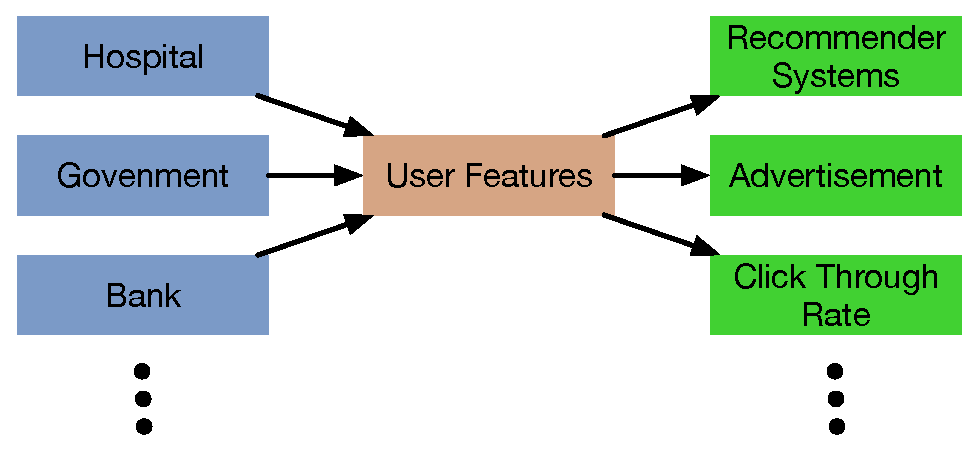
\includegraphics[width=3.2in]{figures/application.eps}
%     \caption{Applying Sensitive User Features to Other Applications}
%     \label{fig:application}
%     \vspace{-5mm}
% \end{figure}


